\documentclass{article}

\title{Metodi Numerici per l'Informatica}
\author{Anthony}
\date{14 mar 2023}

\usepackage{amssymb}
\usepackage{amsmath}
\usepackage{graphicx}

\begin{document}
    \maketitle

    \section{Regolarizzazione: introduzione}
        Abbiamo osservato problemi di fitting del tipo $y_i = ax_i + b$ che sono formalizzati come il seguente problema di minimizzazione:
        \[ \min_{a,b \in \mathbb{R}} \sum_{i=1}^n (y_i - ax_i - b)^2 \]
        Abbiamo anche osservato che possiamo effettuare la regressione polinomiale in modo analogo. Ricordiamo che la regressione polinomiale 
        è lineare nei parametri ma polinomiale rispetto ai dati:
        \[ y_i = b + \sum_{j=1}^k a_j x_i^j \quad \forall i = 1, \dots, n \]
        Usando la notazione matriciale, l'errore quadratico medio è scritto come segue:
        \[ \ell(\mathbf{\theta}) = \Vert \mathbf{y} - \mathbf{X\theta} \Vert_2^2 \]
        settando il gradiente rispetto a $\mathbf{\theta}$ pari a zero e risolvendo per $\mathbf{\theta}$ otteniamo la seguente 
        espressione:
        \[\mathbf{\theta} = (\mathbf{X}^T\mathbf{X})^{-1}\mathbf{X}^T\mathbf{y}\]
        La quale è una soluzione in forma chiusa della regressione lineare. Osserviamo che $\mathbf{\theta}$ non è esattamente uguale a zero, 
        ma minimizza l'uguaglianza. In altre parole, $\mathbf{\theta}$ è una soluzione approssimata che soddisfa la seguente espressione:
        \[\mathbf{X\theta} \approx \mathbf{y}\] 
        In cui l'errore residuo $\Vert \mathbf{y} - \mathbf{X\theta} \Vert_2$ è il più piccolo possibile.
    \section{Equazioni normali}
        Consideriamo il seguente problema lineare:
        \[\mathbf{Ax} = \mathbf{b}\]
        Se esiste una soluzione lineare possiamo scrivere:
        \[\mathbf{x} = \mathbf{A}^{-1}\mathbf{b}\]
        Ma se la soluzione lineare non esiste, dobbiamo risolvere un problema di approssimazione:
        \[\mathbf{Ax} \approx \mathbf{b} \]
        La cui possiamo riscrivere come segue:
        \[\mathbf{A}^T\mathbf{Ax} = \mathbf{A}^T\mathbf{b} \]
        E la soluzione è quindi:
        \[\mathbf{x} = \underbrace{(\mathbf{A}^T\mathbf{A})^{-1}\mathbf{A}^T}_{\text{pseudo-inversa } \mathbf{A}^+}\mathbf{b} \]
        La pseudo-inversa è anche chiamata l'\emph{inversa di Moore-Penrose}. Essa viene utilizzata per risolvere problemi che prevedono un 
        certo scarto quadratico medio.
    \section{Tipi di sistemi lineari}
        Esistono diversi tipi di sistemi lineari. Li identifichiamo con le seguenti categorie:
        \begin{enumerate}
            \item \textbf{Esatto}: $n$ equazioni linearmente indipendenti e $m=n$ parametri. La matrice $\mathbf{A}$ è quindi quadrata.
                \[\text{Problema: } \mathbf{Ax}=\mathbf{b} \quad \text{Soluzione: }\mathbf{x} = \mathbf{A}^{-1}\mathbf{b} \]
            \item \textbf{Sovra-determinato}: $n$ equazioni linearmente indipendenti e $m<n$ parametri. La matrice $\mathbf{A}$ è alta.
                \[\text{Problema: } \mathbf{Ax} \approx \mathbf{b} \quad \text{Soluzione: }\mathbf{x} = (\mathbf{A}^T\mathbf{A})^{-1}\mathbf{A}^T\mathbf{b} \]
            \item \textbf{Sotto-determinato}: $n$ equazioni linearmente indipendenti e $m>n$ parametri. La matrice $\mathbf{A}$ è larga.
                \[\text{Problema: } \mathbf{Ax} \approx \mathbf{b} \quad \text{Soluzione: \textbf{???}} \]
        \end{enumerate}
        In particolare, quando un problema è sotto-determinato, esistono infinite soluzioni. Molte di queste, però, non sono valide. Ad esempio, 
        sarebbero preferibili polinomi che seguono sinuosamente l'andamento dei nostri punti. La \emph{regolarizzazione} è l'aggiunta di 
        informazioni atte a risolvere problemi simili: un problema viene \emph{regolarizzato} quando vengono aggiunte informazioni al 
        problema e quindi ne vengono ridotte le sue soluzioni. 
    \section{La regolarizzazione}
        La regolarizzazione è la chiave per risolvere problemi sotto-determinati aggiungendo più informazioni per restringere le possibili 
        soluzioni del nostro problema. Idea: effettuiamo assunzioni generali e le scriviamo come termini dell'ottimizzazione. \\
        I regolarizzatori portano con loro diversi benefici:
        \begin{itemize}
            \item Impongono un certo comportamento della soluzione, come la sua sparsità o la sua smoothness;
            \item Riducono l'ammontare di dati necessari;
            \item Rendono i problemi di ottimizzazione più semplici da risolvere.
        \end{itemize}

        \subsection{Regolarizzazione di Tikhonov}
            Supponiamo di voler minimizzare l'errore quadratico medio di un certo problema. Ad esso, aggiungiamo un altro termine. In 
            particolare, in questo esempio, aggiungiamo una penalty $L_2$:
            \[ \min_\mathbf{x} \Vert \mathbf{Ax} - \mathbf{b} \Vert_2^2 + \alpha \Vert \mathbf{x} \Vert_2^2 \]
            Per qualche $\alpha > 0$. In questo esempio, stiamo cercando il vettore $\mathbf{x}$ che minimizzi il risultato dell'espressione 
            a sinistra e dell'espressione a destra. \\
            \textbf{Oss:} La $\mathbf{x}$ che comprende tutti zeri minimizza la penalty, ma non l'espressione a sinistra. Difatti, se $\alpha \to 0$
            non stiamo affatto regolarizzando. Se $\alpha \to \infty$, invece, non stiamo tenendo conto dei dati, ovvero delle $\mathbf{x}$. Nel caso 
            generale, dobbiamo scegliere un $\alpha$, risolvere il problema e osservare la soluzione. In caso essa non ci piaccia, trovare un altro 
            $\alpha$. \\
            La funzione ottenuta è convessa in $\mathbf{x}$; possiamo calcolarne il gradiente e porlo uguale a zero:
            \[ \nabla_\mathbf{x} ( \Vert \mathbf{Ax} - \mathbf{b} \Vert_2^2 + \alpha \Vert x \Vert_2^2) = \mathbf{0}\]
            Per linearità del gradiente otteniamo:
            \[ \nabla_\mathbf{x}  \Vert \mathbf{Ax} - \mathbf{b} \Vert_2^2 + \alpha \nabla_\mathbf{x} \Vert x \Vert_2^2 = \mathbf{0}\]
            \[ = 2\mathbf{A}^T\mathbf{Ax} - 2\mathbf{A}^T\mathbf{b} + 2\alpha\mathbf{x} = 0\]
            \[ = \mathbf{A}^T\mathbf{Ax} - \mathbf{A}^T\mathbf{b} + \alpha\mathbf{x} = 0\]
            \[ = \mathbf{A}^T\mathbf{Ax} + \alpha\mathbf{x} =  \mathbf{A}^T\mathbf{b} \]
            \[ = (\mathbf{A}^T\mathbf{A} + \alpha \mathbf{I})\mathbf{x} = \mathbf{A}^T\mathbf{b}\]
            La soluzione è quindi scalata rispetto ad $\alpha$ ed è applicabile anche per problemi sovra-determinati. Per introdurre la 
            regolarizzazione di Tikhonov tutto ciò che dobbiamo fare è aggiungere $\alpha$ per la diagonale di $\mathbf{A}^T\mathbf{A}$. 
            Questo procedimento è anche chiamato \emph{ridge regression}.

            \subsubsection{Esempio: deblurring}
                Supponiamo di voler ripristinare un'immagine sfocata nella sua versione originale.
                \begin{center}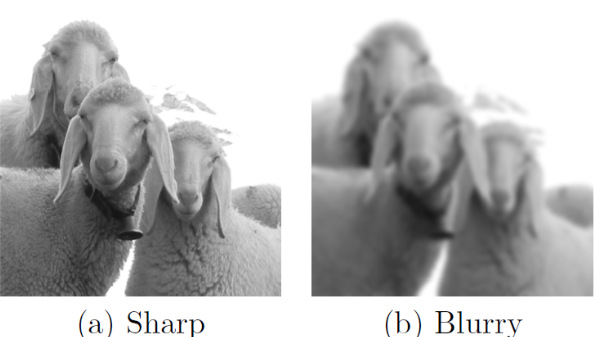
\includegraphics[width=9cm]{tikhonov_example.png}\end{center}
                La nostra 
                incognita è $\mathbf{x}$, l'immagine non sfocata, mentre conosciamo $\mathbf{x_{\text{blurry}}}$, l'immagine sfocata, e $\mathbf{G}$, ovvero 
                la mappa lineare che ha sfocato l'immagine. Questo problema è risolvibile con la regolarizzazione di Tikhonov ai minimi quadrati, a patto che 
                sappiamo quale operatore abbia sfocato la foto:
                \[\min_\mathbf{x} \Vert \mathbf{x}_{\text{blurry}} - \mathbf{Gx} \Vert_2^2 + \alpha \Vert \mathbf{x} \Vert_2^2 \]
        \subsection{Norme $L_p$}
            In generale, possiamo applicare diverse norme per la regolarizzazione, ad esempio la norma $L_p$:
            \[ \min_x \Vert \mathbf{Ax} - \mathbf{b} \Vert_2^2 + \alpha \Vert \mathbf{x} \Vert_p^p \]
            $p$ può essere qualsiasi numero:
            \[\Vert \mathbf{x} - \mathbf{y} \Vert_p = (|x_1 - y_1|^p + |x_2 - y_2|^p)^\frac{1}{p}\]
            Generalizzando a $\mathbb{R}^k$:
            \[\Vert \mathbf{x} - \mathbf{y} \Vert_p = (\sum_{i=1}^k |x_i - y_i|^p)^\frac{1}{p}\]
            Questa definizione esprime il concetto di \emph{distanza $L_p$} tra i vettori in $\mathbb{R}^k$.

            \newpage 

            \paragraph{Circonferenza unitaria}
                Diamo un'occhiata alla circonferenza unitaria applicando diverse norme $L_p$:
                \begin{center}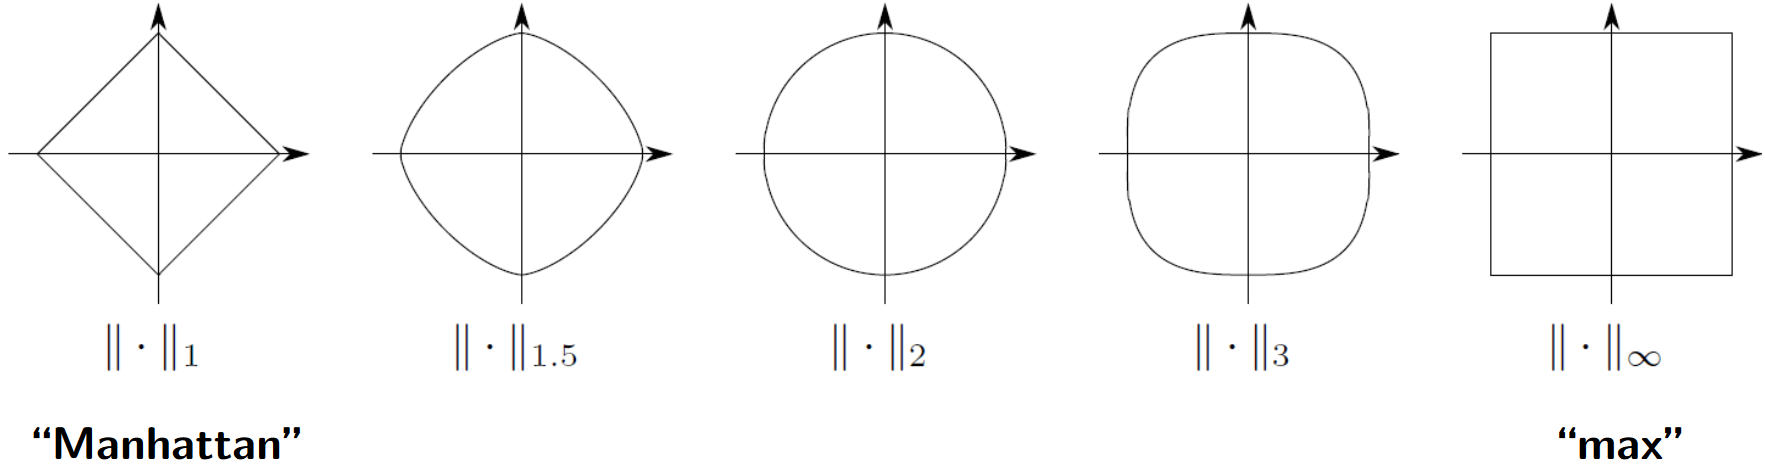
\includegraphics[width=12cm]{lp_norms.png}\end{center}
                Ogni norma $\Vert \cdot \Vert_p$ esprime una \emph{penalty} diversa.
        
        \subsection{Applicazione di Tikhonov con norme diverse}
            Tikhonov esprime un problema di minimizzazione, per cui dalla $\mathbf{x}$ dell'espressione ci aspettiamo che i valori 
            siano piccoli e che i valori grandi siano scoraggiati. In particolare, l'applicazione di Tikhonov con la norma $L_2$ incoraggia 
            ad avere valori tra $0$ e $\pm1$. A seconda della decisione di $p$, i valori di $\mathbf{x}$ saranno penalizzati differentemente.
            \begin{center}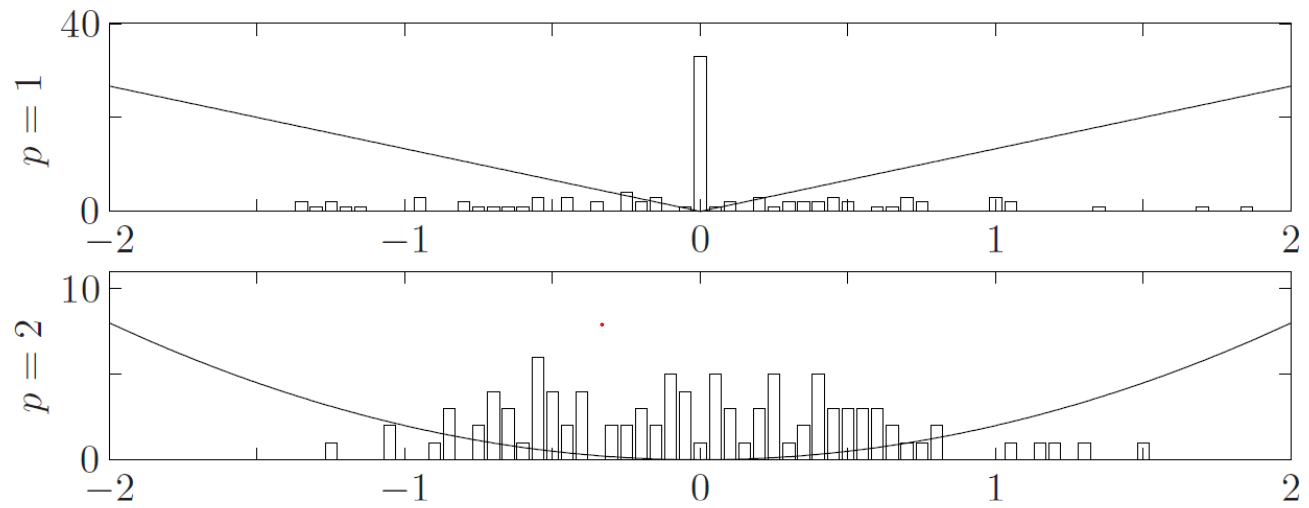
\includegraphics[width=12cm]{tikhonov_l1l2.png}\end{center}
            Possiamo osservare che la norma $L_1$ tende a preferire soluzioni sparse, ovvero sono presenti molti zeri nella soluzione, questo 
            perché tutti i valori prendono una penalty pari al valore stesso.
        
        \subsection{Soluzioni sparse}
            Abbiamo osservato che la regolarizzazione con la norma $L_1$ è un'euristica per trovare soluzioni sparse. Ad esempio, consideriamo 
            il seguente problema:
            \[\min_\mathbf{x} \Vert \mathbf{Ax} - \mathbf{b} \Vert_2^2 + \alpha \Vert \mathbf{x} \Vert_1 \]
            Possiamo osservare che:
            \begin{itemize}
                \item Per $\alpha \approx 0$, questo problema è equivalente al problema dei minimi quadrati.
                \item Per $\alpha \gg 0$, la soluzione $\mathbf{x}$ conterrà molti zeri, e quindi sarà sparsa
                \item Se $\alpha$ è un valore meno estremo, stiamo facendo un compromesso tra la fedeltà dei dati e la sparsità di $\mathbf{x}$. 
            \end{itemize}
            Tale problema non è differenziabile per la norma $L_1$. Non possiamo semplicemente computare il gradiente e settarlo a zero 
            per trovare una soluzione, ma dobbiamo necessariamente approssimare il problema.


        \subsection{Approssimazione di funzioni non differenziabili}
            Proviamo ad applicare la norma $L_1$ a un vettore 1-dimensionale $ \mathbf{x} = \begin{pmatrix}
                x
            \end{pmatrix}$ la sua norma $L_1$ sarà della forma:
            \[f(\mathbf{x}) = |x|\]
            Tale funzione non è differenziabile, ma possiamo riscriverla come segue:
            \[f(\mathbf{x}) = \sqrt{|x|^2}\]
            che ancora non è differenziabile. Però possiamo \emph{ammorbidire} l'angolo del grafico aggiungendo $\epsilon$ molto piccolo:
            \[f(\mathbf{x}) \approx \sqrt{|x|^2} + |\epsilon| \]
            Questa espressione è un'approssimazione della norma $L_1$ di $\mathbf{x}$ ed è differenziabile. Ciò rende possibile 
            la differenziazione di valori assoluti di cui non possiamo fare a meno.

        \subsection{Problemi sparsi}
            Finora abbiamo osservato soluzioni sparse a partire da un problema denso. In particolare, una matrice $\mathbf{A}$ è densa 
            se la maggior parte dei numeri è diversa da zero. Se $\mathbf{A}$ non è densa, allora è sparsa. Consideriamo il seguente problema:
            \[\min_\mathbf{x} \Vert \mathbf{Ax} - \mathbf{b} \Vert_p^p + \alpha\rho(\mathbf{x}) \quad p\geq1, \alpha \geq 0, \text{una funzione regolarizzatrice }\rho\]
            Se la matrice $\mathbf{A}$ è sparsa, allora il problema si dice \emph{problema sparso}. Ad esempio, la matrice $\mathbf{A}$ 
            potrebbe essere una matrice tridiagonale:
            \[\mathbf{A} = \begin{pmatrix}
                v_1 & w_1 & & & & \\
                u_2 & v_2 & w_2 & & & \\
                & u_3 & v_3 & w_3 & & \\
                & & \ddots & \ddots & \ddots & \\
                & & & u_{n-1} & v_{n-1} & w_{n-1} \\
                & & & & u_n & v_n 
            \end{pmatrix}\]

            \paragraph{I grafi} I grafi sono un altro esempio di problema sparso. Ricordiamo che un grafo può esser rappresentato attraverso 
            una matrice di adiacenza: possiamo inserire un 1 in posizione $i,j$ se il nodo $i$ è connesso al nodo $j$, 0 altrimenti. 
            Se il grafo non è particolarmente connesso, la matrice sarà sparsa.
            
            \paragraph{Problemi sparsi: conclusione}In generale, è bene avere un problema sparso poiché esistono algoritmi ad hoc molto efficienti.

    \section{Smoothing}
        Consideriamo il seguente problema: abbiamo un'immagine $\mathbf{x}$ e desideriamo sfocarla. Una soluzione a questo problema 
        prevede il calcolo del problema di minimizzazione e come penalty viene aggiunta la norma del gradiente di $\mathbf{x}$ pesata 
        da un certo $\alpha$:
        \[ \min_\mathbf{x} \Vert \mathbf{y} - \mathbf{x} \Vert_2 + \alpha \Vert \nabla \mathbf{x} \Vert_2^2 \]
        Intuitivamente, la norma $L_2$ promuove soluzioni \emph{smooth}.
        \subsection{Smoothing quadratico}
            Esprimiamo termini della regolarizzazione come $\Vert \mathbf{Dx} \Vert$ in cui $\mathbf{D}$ è un qualche operatore di differenziazione. 
            $\Vert \mathbf{Dx} \Vert$ rappresenta una misura della \emph{variazione} o \emph{smoothness} di $\mathbf{x}$:
            \[\min_\mathbf{x} \underbrace{\Vert \mathbf{Ax} - \mathbf{b} \Vert_2^2}_\text{data term} + \alpha \underbrace{\Vert \mathbf{Dx} \Vert_2^2}_\text{smoothness}\]
            Per esempio, assumiamo che $\mathbf{x} \in \mathbb{R}^n$ rappresenta una funzione in $n$ punti. La sua derivata può esser 
            approssimata come $\mathbf{\Delta x}$, in cui $\mathbf{\Delta}$ è la seguente mappa lineare:
            \[\mathbf{\Delta} = \begin{pmatrix}
                -1 & 1 & 0 & \dots & 0 & 0 & 0 \\
                0 & -1 & 1 & \dots & 0 & 0 & 0 \\
                \vdots & \vdots & \vdots & & \vdots & \vdots & \vdots \\
                0 & 0 & 0 & \dots & -1 & 1 & 0 \\
                0 & 0 & 0 & \dots & 0 & -1 & 1
            \end{pmatrix}\]

            \subsubsection{Denoising}
                Un'applicazione è quella del denoising di un segnale audio. Supponiamo ci sia dato un segnale audio corrotto $\mathbf{x}_\text{cor}$ 
                e vogliamo togliere il rumore dal segnale. Ottimizziamo quindi il seguente problema dello smoothing quadratico:
                    \[ \min_\mathbf{x} \Vert \mathbf{x} - \mathbf{x}_\text{cor} \Vert_2^2 + \alpha \Vert \mathbf{\Delta x} \Vert_2^2\]
                con $\mathbf{\Delta}$ definito come definito più sopra. Se il segnale originale è smooth, lo smoothing quadratico funziona bene tuttavia 
                se consideriamo il seguente segnale rumoroso:
                \begin{center}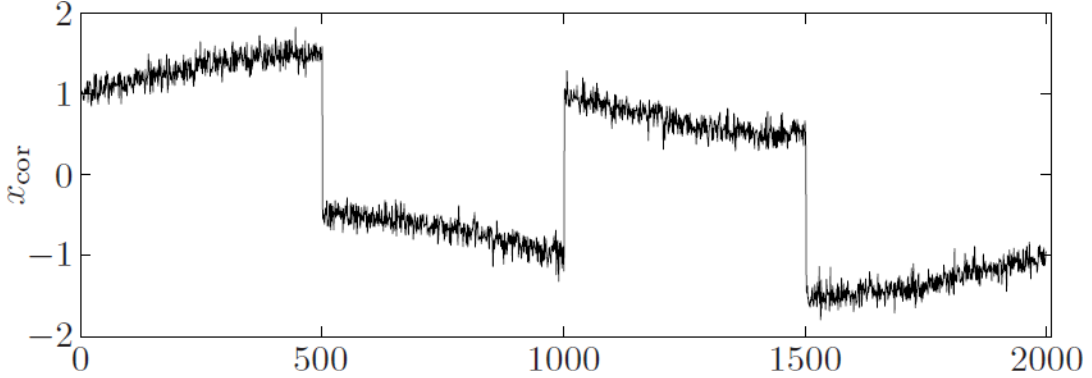
\includegraphics[width=10cm]{onda_quadra.png}\end{center}
                lo smoothing quadratico tratterà i vari salti di frequenza come rumore, attenuandoli:
                \begin{center}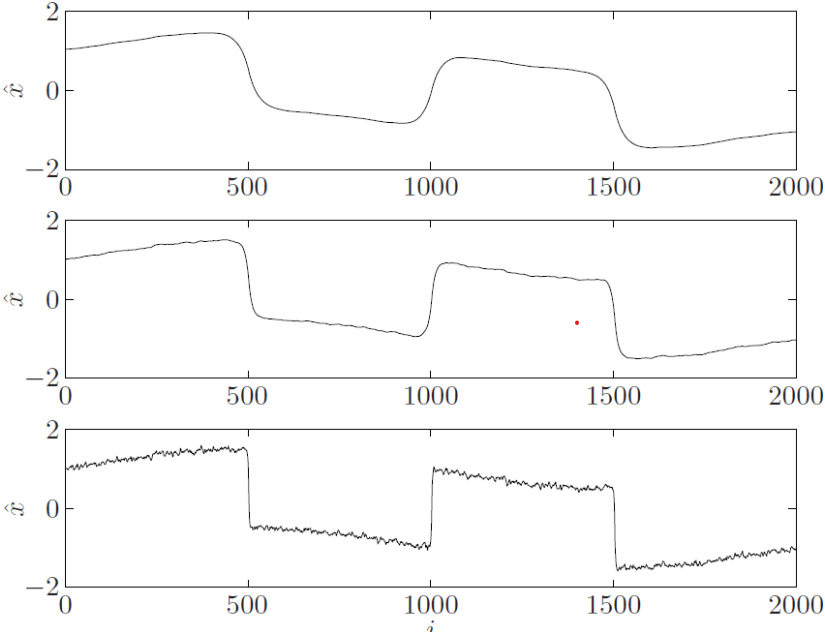
\includegraphics[width=10cm]{onda_quadra_l2.png}\end{center}
                Per prevenire ciò, consideriamo la seguente funzione di smoothing:
                \[ \Vert \mathbf{\Delta x} \Vert_1 = \sum_{i=1}^{n-1} | x_{i+1} - x_i |\]
                E quindi il problema aggiornato:
               \[ \min_\mathbf{x} \Vert \mathbf{x} - \mathbf{x}_\text{cor} \Vert_2^2 + \alpha \Vert \mathbf{\Delta x} \Vert_1\]
               Come abbiamo già detto,utilizzare la norma $L_1$ corrisponde a trovare soluzioni sparse, per cui favorisce la sparsità del
               gradiente; qui non vogliamo affatto valori smooth. All'aumentare di $\alpha$ collasseremo in una retta. 
                \begin{center}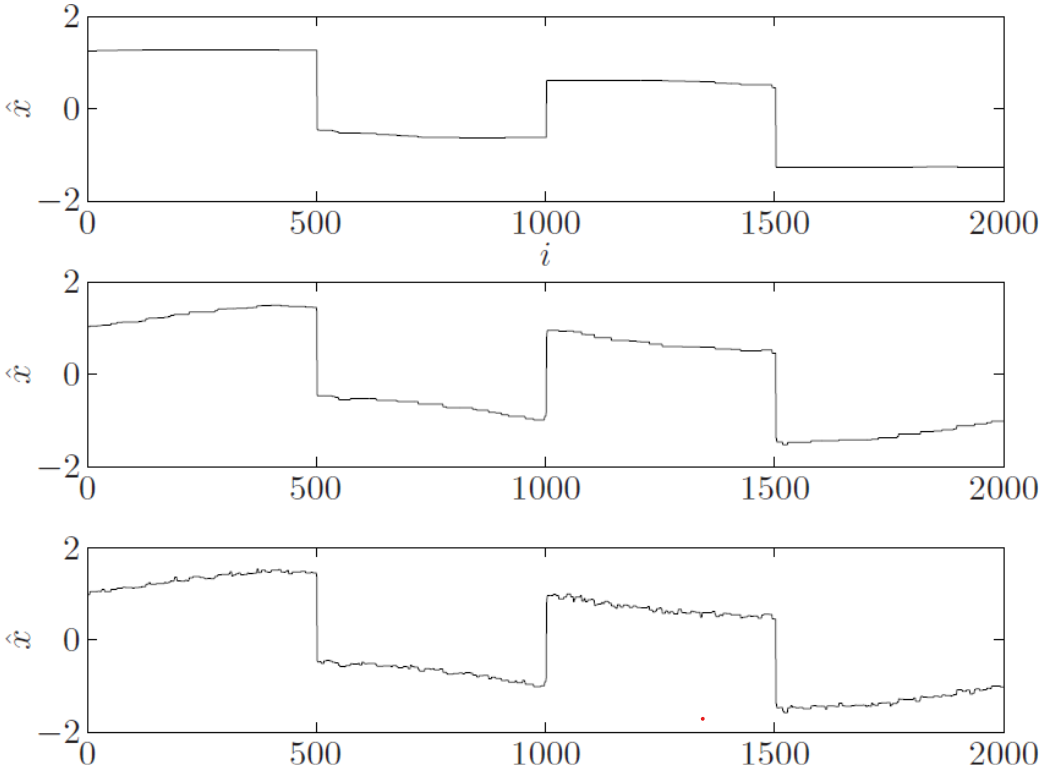
\includegraphics[width=10cm]{onda_quadra_l1.png}\end{center}
                

\end{document}